%%%%%%%%%%%%%%%%%%%%%%%%%%%%%%%%%%%%%%%%%%%%%%%%%%%%%%%%%%%%%
%% Begin exercise %%
%%%%%%%%%%%%%%%%%%%%%%%%%%%%%%%%%%%%%%%%%%%%%%%%%%%%%%%%%%%%%

\ex{Combined step-up / step-down converters}

%%%%%%%%%%%%%%%%%%%%%%%%%%%%%%%%%%%%%%%%%%%%%%%%%%%%%%%%%%%%%
%% Task 1: Inverting buck-boost converter %%
%%%%%%%%%%%%%%%%%%%%%%%%%%%%%%%%%%%%%%%%%%%%%%%%%%%%%%%%%%%%%
\task {Inverting buck-boost converter}
An inverting buck-boost converter (see \autoref{fig:Inverting buck-boost converter}) is used to generate the negative supply voltage of a control electronics. The input voltage is specified as $U_\mathrm{1}=\SI{18}{\volt}$, the output voltage is regulated to $U_\mathrm{2}=\SI{12}{\volt}$. The output power can vary in the range $P_\mathrm{2} = \SI{2}{\watt} \, \dots \, \SI{15}{\watt}$.

\begin{figure}[htb]
    \begin{center}
        \begin{circuitikz}[european currents,european resistors,american inductors]
            \draw 
                    % Base coordinates
                    (0,0) coordinate (jU1v)
                    (0,-3) coordinate (jU1g)
                    % Add components
                    % Add primary source U1
                    (jU1v) to [V,v_=$U_1$] (jU1g)
                    % Add current symbol
                    (jU1v) to [short,i^>=$i_\mathrm{1}$(t)] (1,0)
                    % Add T1 with Control
                    (jU1v) ++(2,0) node[nigfete,rotate=90](Trans1){} -- ++(2.5,0) coordinate(T1)
                    % At transistor label T1
                    (Trans1)  node[anchor=south,color=black]{$T_1$}                    
                    % Short horizontal line
                    (jU1v) to [short,-] (Trans1.D)
                    % Add junction point for inductor
                    (T1) to [short,-*] ++(0,0) coordinate (jLv)
                    % Add junction point for P-buck diode
                    (jLv) ++(0,-3) coordinate (jLg)
                    % Add inductance
                    (jLv) to  [L=$L$] (jLg)
                    % Add current IL symbol
                    (jLv)  to [short,i^>=$i_\mathrm{L}$(t)] (4.5,-0.7)
                    % Continue horizontal line
                    (jLv) to  [short,-] ++ (1.5,0) coordinate (jPtv)
                    % Continue vertical line
                    (jPtv) to  [short,-, crossing] ++ (0,-6) coordinate (jPtg)
                    % Add positive Diode connection point
                    (jPtg)  ++ (3,0) coordinate  (jDP)
                    % Add Diode
                    (jDP) to  [D-,l^=$D$] (jPtg)
                    % Add current Diode
                    (jPtg)  to [short,i^<=$i_\mathrm{D}$(t)] (7,-6)
                    % Add junction point for P-buck diode
                    (jDP) to [short,-*] ++(0,-0) 
                    % Add junction point for capacitor
                    (jDP)  ++(0,3) coordinate (jCv)                    
                    % Add line to secondary source U2
                    (jDP) to  [short,-] ++ (2,0) coordinate (jU2g)
                    % Add positive connection point
                    (jU2g) ++(0,3) coordinate (jU2v)                    
                    % Add secondary source U2
                    (jU2v)  to [V=$U_2$] (jU2g)
                    % Add current I2
                    (jCv)  to [short,i^>=$i_\mathrm{2}$(t)] (11,-3)
                    % Add line to capacitor
                    (jU2v)  to [short,-*] (jCv)
                    % Add capacitor
                    (jCv)  to [C=$C_2$] (jDP)
                    % Add current capacitor
                    (jCv)  to [short,i^>=$i_\mathrm{C}$(t)] (9,-4)
                    % Add horizontal from C to L
                    (jCv) to [short,-*] (jLg)

                    % Connect U1
                    (jLg) to [short,-] (jU1g)
           ;
        \end{circuitikz}
    \end{center}
    \caption{Inverting buck-boost converter.}
    \label{fig:Inverting buck-boost converter}
\end{figure}


\subtask{The system should operate at boundary conduction mode (BCM)   throughout the entire output power range. How should the inductance be selected so that the switching frequency is always above the hearing threshold $f_\mathrm{s}=\SI{20}{\kilo\hertz}$?}

\begin{solutionblock}
The $\Delta$ is an approximation of the total differential using a difference equation with the differences $\Delta$. This results in the component differential equations becoming average value equations. The nabla operator is not understood here due to the $\Delta$.
    \begin{equation}
        U_{\mathrm{1}} = \overline u_{\mathrm{L}} = L \frac{\Delta i_{\mathrm{L}} }{\Delta t}. 
    \end{equation}
\begin{equation}
    D = \frac{U_\mathrm{2}}{U_\mathrm{1}+U_\mathrm{2}} = \frac{\SI{12}{\volt}}{\SI{18}{\volt}+\SI{12}{\volt}} = 0.4
\end{equation}
BCM is assumed. A current $I_\mathrm{2}$ is only present when the transistor is open, otherwise the diode blocks. This is taken into account in the following equation as the duty cycle $D = 0.6$ is used for $T_\mathrm{off}$. The equation thus looks as follows:
\begin{equation}
    I_\mathrm{2,min} = \frac{P_\mathrm{2}}{U_\mathrm{2}} \frac{1}{D}=\frac{\SI{15}{\watt}}{\SI{12}{\volt}}\frac{5}{3}=\SI{2.083}{\volt}
\end{equation}
The maximum current at BCM $\Delta i_{\mathrm{L}}$ is twice  $I_\mathrm{2,min}$:
\begin{equation}
    \Delta i_{\mathrm{L}} = 2  I_\mathrm{2,min} = \SI{4.16}{\ampere}.
\end{equation}
Delta $\Delta t$ can also be expressed as:
\begin{equation}
    \Delta t = \frac{D}{f_\mathrm{s}}.
\end{equation}
This expression can now be used in the inductance equation. The inductance can therefore be determined using the following equation:
\begin{equation}
    L = \frac{\Delta t  \overline u_{\mathrm{L}}}{\Delta i_{\mathrm{L}}}= \frac{D \overline u_{\mathrm{L}}}{f_\mathrm{s}\Delta i_{\mathrm{L}}}= \frac{D U_{\mathrm{1}}}{f_\mathrm{s}\Delta i_{\mathrm{L}}} = \frac{0.4 \cdot \SI{18}{\volt}}{\SI{20}{\kilo\hertz}\cdot \SI{4.16}{\ampere }} = \SI{86.4}{\micro\henry}.
\end{equation}

\end{solutionblock}
\subtask{In what value range does the switching frequency $f_\mathrm{s}$ vary considering the inductance choice from the previous subtask and the given output power range?}

 \begin{solutionblock}
     The inductance equation is used again for this task:
     \begin{equation}
        L = \frac{\Delta t \overline u_{\mathrm{L}}}{\Delta i_{\mathrm{L}}}= \frac{D \overline u_{\mathrm{L}}}{f_\mathrm{s}\Delta i_{\mathrm{L}}}
     \end{equation}
     This equation can be converted to $f_\mathrm{s}$ and used to determine the frequency as follows:
     \begin{equation}
        f_\mathrm{s} = \frac{DU_{\mathrm{1}}}{L\Delta i_{\mathrm{L}}} \label{equation 1.8}
     \end{equation}
      
As the output power is specified as a value range, the highest and lowest values can be used. The lowest and highest current should be determined from these two values, from which the value range of the frequency $f_\mathrm{s}$ can then be determined. Here the inverse converter is considered on the output side and therefore a duty cycle $D = 0.6$ is used again. The following equations can be derived from this:

     \begin{equation}
        I_\mathrm{2,min}= \frac{P_\mathrm{2}}{U_\mathrm{2}}\frac{1}{D}=\frac{\SI{2}{\watt}}{\SI{12}{\volt}}\frac{5}{3}=\SI{0.278}{\volt}
     \end{equation}
     \begin{equation}
        I_\mathrm{2,max}= \frac{P_\mathrm{2}}{U_\mathrm{2}}\frac{1}{D}=\frac{\SI{15}{\watt}}{\SI{12}{\volt}}\frac{5}{3}=\SI{2.0833}{\volt}
     \end{equation}
     Now we can use these two terms in \ref{equation 1.8}:
     \begin{equation}
        f_\mathrm{P,max}=\frac{0.4\cdot\SI{18}{\volt}}{\SI{86.4}{\micro\henry}\cdot 2\cdot \SI{0.278}{\volt}}=\SI{150}{\kilo \hertz}
     \end{equation}
     \begin{equation}
        f_\mathrm{P,min}=\frac{0.4\cdot\SI{18}{\volt}}{\SI{86.4}{\micro\henry}\cdot 2\cdot \SI{2.0833}{\volt}}=\SI{20}{\kilo \hertz}
     \end{equation}
     The switching frequency $f_\mathrm{s}$ varies in the range from $\SI{20}{\kilo \hertz} \, \dots \, \SI{150}{\kilo \hertz}$.
 \end{solutionblock}

 \subtask{What is the peak value $\hat i_1=\max\{i_1(t)\}$ of the transistor current?}
 \begin{solutionblock}
    As the maximum current through the transistor is the current $i_1$, these values are the same. Since the BCM is considered in this circuit, the maximum current is the peak current, which corresponds to the value of $\SI{4.16}{\ampere}$.
 \end{solutionblock}

 \subtask{How does the duty cycle $D$ change with the output power? Calculate the duty cycle values and the absolute values of the transistor switch-on times $T_\mathrm{on} = D T_\mathrm{s}$ for minimum and maximum output power.}
 \begin{solutionblock}
 The following applies to the switching period $T_\mathrm{s}$ for the respective services:  
 \begin{equation}
    T_\mathrm{s} = \frac{1}{f_\mathrm{s}}. \label{switching frequency}
 \end{equation}
 The different switching frequencies can now be inserted into \ref{switching frequency}:
 \begin{equation}
    T_\mathrm{s,min}(\SI{2}{\watt}) = \frac{1}{\SI{150}{\kilo \hertz}}= \SI{6.67}{\micro \s}
 \end{equation}
 \begin{equation}
    T_\mathrm{s,max}(\SI{15}{\watt}) = \frac{1}{\SI{20}{\kilo \hertz}}= \SI{50}{\micro \s}.
 \end{equation}
 The absolute values of the transistor switch-on times can be determined using the following equation
 \begin{equation}
    T_\mathrm{on} = D T_\mathrm{s}. \label{absolut value switch-on-times}
 \end{equation}
 The different switching periods can now be inserted into \ref{absolut value switch-on-times}:
 \begin{equation}
    T_\mathrm{on,min}(\SI{2}{\watt}) = 0.4 \cdot \SI{6.67}{\micro \s} = \SI{2.67}{\micro \s}
 \end{equation}
 \begin{equation}
    T_\mathrm{on,max}(\SI{15}{\watt}) = 0.4 \cdot \SI{50}{\micro \s}= \SI{20}{\micro \s}.
 \end{equation}
 \end{solutionblock}

 \subtask{Sketch the course of the inductor current $i_\mathrm{L}(t)$  for minimum and maximum output power.}
\begin{solutionblock}
    \begin{solutionfigure}[htb]
    \centering
    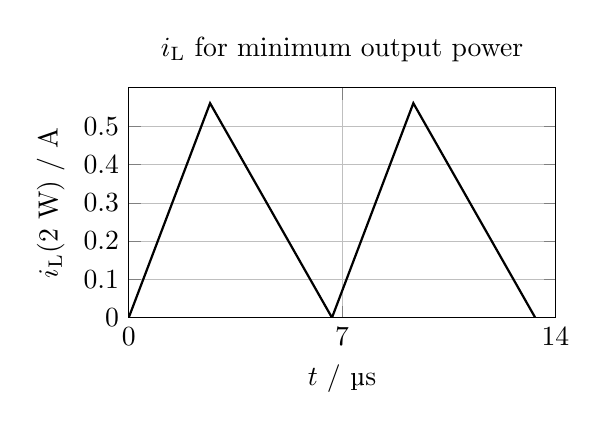
\begin{tikzpicture}
    \begin{axis}[
        width=7cm, height=4.5cm,
        grid=both,
        major grid style={line width=.2pt,draw=gray!50},
        minor grid style={line width=.1pt,draw=gray!20},
        xlabel={$t$ / µs},
        ylabel={$i_\mathrm{L}(\mathrm{2~W})$ / A},
        title={$i_\mathrm{L}$ for minimum output power},
        xmin=0, xmax=14,
        ymin=0, ymax=0.6,
        xtick={0, 7, 14},
        ytick={0, 0.1, 0.2, 0.3, 0.4, 0.5},
        ]
        % Einschaltverhalten graph
        \addplot[
            thick,
            mark=none,
            color=black,
        ] coordinates {
            (0,0) (2.67,0.56) (6.67, 0) (9.34,0.56) (13.34, 0)
        };
    \end{axis}
    \end{tikzpicture} 
    \hspace{1cm} % Abstand zwischen den beiden Diagrammen
    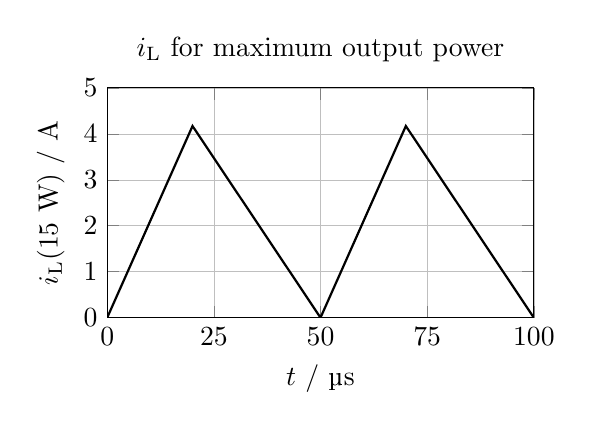
\begin{tikzpicture}
    \begin{axis}[
        width=7cm, height=4.5cm,
        grid=both,
        major grid style={line width=.2pt,draw=gray!50},
        minor grid style={line width=.1pt,draw=gray!20},
        xlabel={$t$ / µs},
        ylabel={$i_\mathrm{L}(\mathrm{15~W})$ / A},
        title={$i_\mathrm{L}$ for maximum output power},
        xmin=0, xmax=100,
        ymin=0, ymax=5,
        xtick={0, 25, 50, 75, 100},
        ytick={0, 1, 2, 3, 4, 5},
        ]
        % Ausschaltverhalten graph
        \addplot[
            thick,
            mark=none,
            color=black,
        ] coordinates {
            (0,0) (20, 4.17) (50, 0) (70, 4.17) (100, 0)
        };
    \end{axis}
    \end{tikzpicture}
    \caption{Display of the inductance current $i_\mathrm{L}$ for minimum and maximum output power.}
    \label{fig:InductorCurrentEx03}
    \end{solutionfigure}   
\end{solutionblock}
    
 \subtask{At which operating point does the maximum output voltage ripple $\Delta u_\mathrm{2}$ occur (assumption: the load draws a constant current)?} 

 \subtask{How high should the output capacitance be selected to ensure $\Delta u_\mathrm{2} < 0.02 \cdot U_\mathrm{2}?$}

 \subtask{What is the maximum effective value $i_\mathrm{C,RMS}$ of the output capacitor current?}

 \subtask{Sketch the curves of the voltage $u_\mathrm{T}(t)$ at the power transistor and the current $i_\mathrm{D}(t)$ in the output diode for $P_\mathrm{2}=\SI{2}{\watt}$. What is the maximum blocking voltage of the transistor?}

%%%%%%%%%%%%%%%%%%%%%%%%%%%%%%%%%%%%%%%%%%%%%%%%%%%%%%%%%%%%%
%% Task 2: Boost-Buck converter and SEPIC topology
%%%%%%%%%%%%%%%%%%%%%%%%%%%%%%%%%%%%%%%%%%%%%%%%%%%%%%%%%%%%%

\task {Boost-buck converter and SEPIC topology}

The supply of a plasma coating system is realized by a boost converter followed by a buck converter acccording \autoref{fig:ex03_boost_buck_converter} (with common capacitance).
The converter is connected to a voltage $U_\mathrm{1}$ and provides a variable output voltage $U_\mathrm{2}$. The parameters are displayed in \autoref{table:ParametersOfBoostBuckConverter}.
\vspace{2em}\par

\par
% Schematic of Buck Boost Converter cascade

\begin{figure}[htb]
    \begin{center}
        \begin{circuitikz}[european currents,european resistors,american inductors]
            \draw 
                    % Base coordinates
                    (0,0) coordinate (jU1v)
                    (0,-3) coordinate (jU1g)
                    % Add primary source U1
                    (jU1v) to [V=$U_1$] (jU1g)
                    % Add line to L1
                    (jU1v) to [short,-] ++ (0.5,0) coordinate (jL1v)
                    % Add Inductance L1
                    (jL1v) to  [L, l=$L_1$] ++ (3,0) coordinate (jT1v)
                    % Add arrow and Text
                    ++(-0.5,0) node[currarrow](IL1){}
                    (IL1)  node[anchor=south,color=black]{$i_\mathrm{L1}$}
                    % Add junction for T1
                    (jT1v) to [short,-*] ++(0,0)
                    % Add coordinate for Transistor
                    (jT1v) ++(0,-3) coordinate (jT1g)
                    % Add transistor T2
                    (jT1v) ++ (0,-1.5) node[nigfete](Trans1){}
                    % At transistor label T2
                    (Trans1)  node[anchor=west,color=black]{$T_1$}                     
                    % Connect Transistor
                    (jT1v) to [short,-] (Trans1.D)
                    (jT1g) to [short,-] (Trans1.S)
                    (Trans1.G) to [sqV] ++(-1,0)
                    % Add diode D1
                    (jT1v) to  [D,l=$D_1$] ++ (2,0) coordinate (jCv)
                    % Add junction for C
                    (jCv) to [short,-*] ++(0,0)
                    % Add coordinate jCv and jCg
                    (jCv)  ++(0,-3) coordinate (jCg)
                    % Add  capacitor C
                    (jCv)  to [C, l=$C$] (jCg)
                    % Add current symbol and T2 with Control
                    (jCv) ++(2,0) node[nigfete,rotate=90](Trans2){} -- ++(2.5,0) coordinate(T2)
                    (Trans2.G)  to [sqV] ++(0,-1)
                    % At transistor label T2
                    (Trans2)  node[anchor=south,color=black]{$T_2$}                    
                    % Short horizontal line
                    (jCv) to [short,-] (Trans2.D)
                    % Add junction point for M-buck diode
                    (T2) to [short,-*] ++(0,0) coordinate (jD2M)
                    % Add junction point for diode D2
                    (jD2M) ++(0,-3) coordinate (jD2P)
                    % Add diode D2
                    (jD2P) to  [D,l=$D_2$] (jD2M)                                      
                    % Add inductor L2
                    (jD2M) to  [L,l^=$L_2$] ++ (3,0) coordinate (jU2v)
                    % Add arrow and Text
                    (jU2v) ++(-0.5,0) node[currarrow](IL2){}
                    (IL2)  node[anchor=south,color=black]{$i_\mathrm{L2}$}
                    % Add coordinate jU2v and jU2g
                    (jU2v) to [short,-] ++(0,-3) coordinate (jU2g)
                    % Add secondary source U2
                    (jU2v) to [V=$U_2$] (jU2g)
                    % Add line and junction to D2
                    (jU2g) to [short,-*] (jD2P)
                    % Add line and junction to C
                    (jD2P) to [short,-*] (jCg)                    
                    % Add line and junction to T1
                    (jCg) to [short,-*] (jT1g)                    
                    % Add line and junction to U1
                    (jT1g) to [short,-] (jU1g)                    
           ;
        \end{circuitikz}
    \end{center}
    \caption{Buck-boost converter circuit.}
    \label{fig:ex02_step_down_with_load_resistor}
\end{figure}

\par
%Table of parameter values 
%%%%%%%%%%%%%%%%%%%%%%%%%%%%%%%%%%%%%%%%%%%%%%%%%%%%%%%%%%%%%%%%%%%%%%%%%%
%  Boost buck converter parameter
%%%%%%%%%%%%%%%%%%%%%%%%%%%%%%%%%%%%%%%%%%%%%%%%%%%%%%%%%%%%%%%%%%%%%%%%%%

\begin{table}[ht]
    \centering  % Zentriert die Tabelle
    \begin{tabular}{llll}
        \toprule
        
        Input voltage: &  $U_{\mathrm{1}} = \SI{380}{\volt}$ & Output voltage: & $U_{\mathrm{2}} = \SI{285}{\volt}$  to $\SI{450}{\volt}$\\ 
        Output power: & $P_{\mathrm{2}} = \SI{3000}{\watt}$ & Switching frequency: & $f_{\mathrm{s}} = \SI{50}{\kilo\hertz}$ \\ 
        \multicolumn{4}{l}{$P_{\mathrm{2}}$ is constant (unless otherwise stated)} \\
        \bottomrule
    \end{tabular}
    \caption{Parameters of the circuit.}  % Beschriftung der Tabelle
    \label{table:Parameters of the buck-boost converter.}
\end{table}

The output voltage is set to the specified value by adjusting the duty cycles $D_\mathrm{1}$ (of transistor $T_\mathrm{1}$) 
and $D_\mathrm{2}$ (of transistor $T_\mathrm{2}$) using a control system. Both transistors operate at the same switching frequency. 
The switching frequency fluctuation of the intermediate circuit voltage and the currents in the inductors can be neglected unless otherwise stated. 
The currents in $L_\mathrm{1}$ and $L_\mathrm{2}$ show a continuous course. Both transistors are operated with the 
same relative duty cycle $D_\mathrm{1}$ = $D_\mathrm{2}$ = $D$.

\subtask{Calculate the duty cycle $D$ range to achieve the stated output voltage $U_\mathrm{2}$ range.}

\begin{solutionblock}
    % Solution
    For the boost-buck converter \eqref{eq:DutyCycleEx03} is to apply:
    \begin{equation}
        \frac{U_\mathrm{2}}{U_\mathrm{1}} = \frac{D} {1-D}
        \hspace{1cm} \rightarrow \hspace{1cm}
        D = \frac{\frac{U_\mathrm{2}}{U_\mathrm{1}}} {1+{\frac{U_\mathrm{2}}{U_\mathrm{1}}}}.
        \label{eq:DutyCycleEx03}
    \end{equation}
    In case of $U_\mathrm{2}$ = $\SI{285}{\volt}$, the duty cycle is determined using \eqref{eq:DutyCycleEx03} as
    \begin{equation}
       \frac{\frac{\SI{285}{\volt}}{\SI{380}{\volt}}} {1+{\frac{\SI{285}{\volt}}{\SI{380}{\volt}}}} = 0.429.
    \end{equation}
\end{solutionblock}


\subtask{Which intermediate circuit voltage $U_\mathrm{0}$ results depending on $U_\mathrm{2}$?}

\begin{solutionblock}
    % Solution
    The first part is the boost converter part. For the output voltage 
    of $\SI{285}{\volt}$, the intermediate circuit voltage $U_\mathrm{0}$ is calculated as
    \begin{equation}
        U_\mathrm{0}=U_\mathrm{1} \frac{1}{1-D} 
        \hspace{1cm} \mathrm{and} \hspace{1cm}  
        \SI{380}{\volt} \frac{1}{1-0.429} = \SI{665}{\volt}.
        \label{eq:DCLinkEx03}        
    \end{equation}
\end{solutionblock}


\subtask{Plot $D$ and $U_\mathrm{0}$ against $U_\mathrm{2}$ and calculate the numerical values for $U_\mathrm{2}=\SI{285}{\volt}$, $U_\mathrm{2}=\SI{380}{\volt}$ and $U_\mathrm{2}=\SI{450}{\volt}$.}

\begin{solutionblock}
    % Solution
    For the plot \eqref{eq:DutyCycleEx03} and \eqref{eq:DCLinkEx03} are used to calculate results in \autoref{table:DutyCycleDCLinkVoltageAtOutputVoltage} 
    and displayed in \autoref{fig:DCLinkVoltageAtOutputVoltage} and \autoref{fig:DutyCycleDCAtOutputVoltage}.

    %Result table
    %%%%%%%%%%%%%%%%%%%%%%%%%%%%%%%%%%%%%%%%%%%%%%%%%%%%%%%%%%%%%%
% Solution table Output voltage-> DC-Link voltage  Duty cycle
%%%%%%%%%%%%%%%%%%%%%%%%%%%%%%%%%%%%%%%%%%%%%%%%%%%%%%%%%%%%%%
\begin{solutiontable}[htb]
    \centering  % Zentriert die Tabelle
    \begin{tabular}{lll}
        \toprule
        \multicolumn{1}{c}{$U_\mathrm{2}$} & \multicolumn{1}{c}{$U_\mathrm{0}$} & \multicolumn{1}{c}{$D$} \\
        \midrule 
        $\SI{285}{\volt}$ & $\SI{665}{\volt}$ & 0.429\\ 
        $\SI{380}{\volt}$ & $\SI{760}{\volt}$ & 0.5 \\ 
        $\SI{450}{\volt}$ & $\SI{830}{\volt}$ & 0.542\\ 
        \bottomrule
    \end{tabular}
    \caption{$D$ and $U_\mathrm{0}$ at $U_\mathrm{2}$.}
    \label{table:DutyCycleDCLinkVoltageAtOutputVoltage}
\end{solutiontable}

    %Plot of DCLinkVoltage
    %%%%%%%%%%%%%%%%%%%%%%%%%%%%%%%%%%%%%%%%%%%%%%%%%%%%%%%%%%%%%%%%%%%%%%%%%%
% Dutycycle and DC-Link voltage versus output voltage
%%%%%%%%%%%%%%%%%%%%%%%%%%%%%%%%%%%%%%%%%%%%%%%%%%%%%%%%%%%%%%%%%%%%%%%%%%

\begin{solutionfigure}[htb]
    \centering
    \begin{minipage}{0.8\textwidth}
        \centering
        \begin{tikzpicture}
            \begin{axis}[,
                    % x/y range adjustment
                    xmin=250, xmax=500,
                    ymin=580, ymax=900,
                    samples=500,
                    axis y line=center,
                    axis x line=middle,
                    extra y ticks=0,
                    % Label text
                    xlabel={$U_\mathrm{2} \text{/V}$},
                    ylabel={$U_\mathrm{0} \text{/V}$},
                    % Label adjustment
                    x label style={at={(axis description cs:1,0)},anchor=west},
                    y label style={at={(axis description cs:-.05,1)},anchor=south},
                    width=0.6\textwidth,
                    height=0.3\textwidth,
                    % x-Ticks                
                    xtick={250,300,350,400,450,800},
                    xticklabels={250,300,350,400,450,800},
                    xticklabel style = {anchor=north},
                    % y-Ticks                
                    ytick={600,650,700,750,800,850},
                    yticklabels={600,,700,,800,},
                    yticklabel style = {anchor=east},
                    % Grid layout                
                    grid=both,
                    grid style={line width=.1pt, draw=gray!10},
                    major grid style={line width=.2pt,draw=gray!50},
                ]
                \addplot[signalalpha, domain=282:450, thick] {x+380};
            \end{axis}
        \end{tikzpicture}
    \end{minipage}
    \caption{Intermediatie circuit voltage versus output voltage.}
    \label{fig:DCLinkVoltageAtOutputVoltage}     
\end{solutionfigure}







    %Plot of duty cycle
    %%%%%%%%%%%%%%%%%%%%%%%%%%%%%%%%%%%%%%%%%%%%%%%%%%%%%%%%%%%%%%%%%%%%%%%%%%
% Dutycycle and DC-Link voltage versus output voltage
%%%%%%%%%%%%%%%%%%%%%%%%%%%%%%%%%%%%%%%%%%%%%%%%%%%%%%%%%%%%%%%%%%%%%%%%%%

\begin{solutionfigure}[htb]
    \centering
    \begin{minipage}{0.8\textwidth}    
        \centering
        \begin{tikzpicture}
            \begin{axis}[,
                    % x/y range adjustment
                    xmin=250, xmax=500,
                    ymin=0.4, ymax=0.65,
                    samples=500,
                    axis y line=center,
                    axis x line=middle,
                    extra y ticks=0,
                    % Label text
                    xlabel={$U_\mathrm{2} \text{/V}$},
                    ylabel={$D$},
                    % Label adjustment
                    x label style={at={(axis description cs:1,0)},anchor=west},
                    y label style={at={(axis description cs:-.05,1)},anchor=south},
                    width=0.6\textwidth,
                    height=0.3\textwidth,
                    % x-Ticks                
                    xtick={250,300,350,400,450,800},
                    xticklabels={250,300,350,400,450,800},
                    xticklabel style = {anchor=north},
                    % y-Ticks                
                    ytick={0.4,0.45,0.5,0.55,0.6},
                    yticklabels={0.4,0.45,0.5,0.55,0.6},
                    yticklabel style = {anchor=east},
                    % Grid layout                
                    grid=both,
                    grid style={line width=.1pt, draw=gray!10},
                    major grid style={line width=.2pt,draw=gray!50},
                ]
                \addplot[signaldelta, domain=282:450, thick] {(x/380)/(1+x/380)};
            \end{axis}
        \end{tikzpicture}
        \end{minipage}
        \caption{Duty cycle versus output voltage.}
    \label{fig:DutyCycleAtOutputVoltage}     
\end{solutionfigure}








\end{solutionblock}

\subtask{What blocking voltage ratings must the transistors $T_\mathrm{1}$ and $T_\mathrm{2}$ and the diodes $D_1$ and
$D_2$ have?}

\begin{solutionblock}
    % Solution
    Based on the schematic \autoref{fig:ex03_boost_buck_converter} the intermediate circuit voltage is to block by the diodes and 
    the transistors within one switching period. The minimum blocking voltage of the component needs to be higher than $U_\mathrm{0}$.
\end{solutionblock}

\vspace{2em}\par
The converter operation continues with $D_\mathrm{1}$ = $D_\mathrm{2}$ = $D$. The input and output inductances 
have the same value $L_\mathrm{1}$ = $L_\mathrm{2}$ = $L$ = $\SI{0.5}{m\henry}$.

\subtask{Derive the input and output current ripple $\Delta i_\mathrm{L_1}$ and $\Delta i_\mathrm{L_2}$ depending on the duty cycle.}

\begin{solutionblock}
    % Solution
    The current ripple depends on the duty cycle, switching period and inductor voltage.
    \eqref{eq:Boostripple} applies to the boost converter stage:
    \begin{equation}
        \Delta i_\mathrm{L1}=\frac{U_\mathrm{1}D}{f_\mathrm{s}L}
        \label{eq:Boostripple}
    \end{equation}
    and \eqref{eq:Buckripple} to the buck converter stage:
    \begin{equation}
        \Delta i_\mathrm{L2}=\frac{\left(U_\mathrm{0}-U_\mathrm{2}\right)D}{f_\mathrm{s}L}.
        \label{eq:Buckripple}
    \end{equation}
\end{solutionblock}

\subtask{To what minimum value can the output power be reduced while still ensuring 
continuous operation across the entire output voltage range 
(i.e., continuous current flow in $L_\mathrm{1}$  and $L_\mathrm{2}$)?}

\begin{solutionblock}
    % Solution
    For the boost stage the power is the product of output voltage
     ($U_\mathrm{0}$) and average current calculated by using \eqref{eq:Boostripple}:
    \begin{equation}
        P_\mathrm{lim,boost}=U_\mathrm{0}\frac{\Delta i_\mathrm{L1}}{2}D.
        \label{eq:PowerBoostripple}
    \end{equation}
    For the buck stage the power is the product of output voltage
    ($U_\mathrm{2}$) and average current calculated by using \eqref{eq:Buckripple}:
    \begin{equation}
        P_\mathrm{lim,buck}=U_\mathrm{2}\frac{\Delta i_\mathrm{L2}}{2}.
        \label{eq:PowerBuckripple}
    \end{equation}
    Entering the values in \eqref{eq:PowerBoostripple} and \eqref{eq:PowerBuckripple} leads to \autoref{table:PowerminInputOutputStage}.
    %Solution table Minimal Power 
    %%%%%%%%%%%%%%%%%%%%%%%%%%%%%%%%%%%%%%%%%%%%%%%%%%%%%%%%%%%%%%
% Solution table Output voltage-> Minimal power
%%%%%%%%%%%%%%%%%%%%%%%%%%%%%%%%%%%%%%%%%%%%%%%%%%%%%%%%%%%%%%
\begin{solutiontable}[htb]
    \centering  % Zentriert die Tabelle
    \begin{tabular}{lll}
        \toprule
        \multicolumn{1}{c}{$U_\mathrm{2}$} & \multicolumn{1}{c}{$P_\mathrm{min,boost}$} 
        & \multicolumn{1}{c}{$P_\mathrm{min,buck}$} \\
        \midrule 
        $\SI{285}{\volt}$ & $\SI{930}{\watt}$ & $\SI{929}{\watt}$\\ 
        $\SI{380}{\volt}$ & $\SI{1444}{\watt}$ & $\SI{1444}{\watt}$ \\ 
        $\SI{450}{\volt}$ & $\SI{1853}{\watt}$ & $\SI{1854}{\watt}$\\ 
        \bottomrule
    \end{tabular}
    \caption{Minimal power necessary for CCM (boost and buck stage).}
    \label{table:PowerminInputOutputStage}
\end{solutiontable}


    The minimal power, which ensuring continuous operation across the entire output voltage range
    yields  $\SI{1854}{\watt}$.
\end{solutionblock}

\subtask{At which value of the output voltage range is this limit reached first on the input side and at which value is it reached first on the output side?}
\begin{solutionblock}
    % Solution
    As displayed in \autoref{table:PowerminInputOutputStage} the minimal power limit is caused by the 
    boost-stage (input side) for output voltage less than 380V. For output voltages greater than 380V 
    the buck-stage (output side) causes the minimal power limit for continuous conduction mode.
\end{solutionblock}

\vspace{2em}\par
For comparison reasons, the single ended primary inductance converter (SEPIC) in \autoref{fig:ex03_SEPIC} shall be considered under similar conditions as an alternative circuit.

% Schematic of Buck Boost Converter cascade

%%%%%%%%%%%%%%%%%%%%%%%%%%%%%%%%%%%%%%%%%%%%%%%%%%%%%%%%%%%%%%%%%%%%%%%%%%
%  Single Ended Primary Inductance Converter Schematic
%%%%%%%%%%%%%%%%%%%%%%%%%%%%%%%%%%%%%%%%%%%%%%%%%%%%%%%%%%%%%%%%%%%%%%%%%%

\begin{figure}[ht]
    \begin{center}
        \begin{circuitikz}[european currents,european resistors,american inductors]
            \draw 
                    % Base coordinates
                    (0,0) coordinate (jU1v)
                    (0,-3) coordinate (jU1g)
                    % Add primary source U1
                    (jU1v) to [V=$U_1$] (jU1g)
                    % Add line to L1
                    (jU1v) to [short,-] ++ (0.5,0) coordinate (jL1v)
                    % Add Inductance L1
                    (jL1v) to  [L, l=$L_1$] ++ (3,0) coordinate (jTv)
                    % Add arrow and Text
                    ++(-0.5,0) node[currarrow](IL){}
                    (IL)  node[anchor=south,color=black]{$i_\mathrm{L}$}
                    % Add junction for Transistor
                    (jTv) ++(0,-3) coordinate (jTg)
                    % Add junction point for Transistor
                    (jTv) to [short,-*] ++(0,0)                    
                    % Add transistor T2
                    (jTv) ++ (0,-1.5) node[nigfete](Trans1){}
                    % At transistor label T2
                    (Trans1)  node[anchor=west,color=black]{$T$}                     
                    % Connect Transistor
                    (jTv) to [short,-] (Trans1.D)
                    (jTg) to [short,-] (Trans1.S)
                    (Trans1.G) to [sqV] ++(-1,0)
                    % Add capacitor C
                    (jTv) to  [C,l=$C$] ++ (2,0) coordinate (jL2v)
                    % Add junction for L2
                    (jL2v) to [short,-*] ++(0,0)
                    % Add coordinate jL2v and jL2g
                    (jL2v)  ++(0,-3) coordinate (jL2g)
                    % Add  L2
                    (jL2v)  to [L, l=$L_2$] (jL2g)
                    % Add Diode
                    (jL2v) to  [D-,l^=$D$] ++ (2,0) coordinate (jU2v) 
                    % Add coordinate jU2v and jU2g
                    (jU2v) to [short,-] ++(0,-3) coordinate (jU2g)
                    % Add secondary source U2
                    (jU2v) to [V=$U_2$] (jU2g)
                    % Add Junction point for jL2g
                    (jU2g) to [short,-*] (jL2g)
                    % Add line and junction point for T1g
                    (jL2g) to [short,-*] (jTg)
                    % Add line to U1g
                    (jTg) to [short,-] (jU1g)
           ;
        \end{circuitikz}
    \end{center}
    \caption{Single ended  primary inductance converter circuit.}
    \label{fig:ex03_SEPIC}
\end{figure}


\subtask{What blocking voltage ratings must the transistors $T_\mathrm{1}$ and the diode $D$ have?}
\begin{solutionblock}
    % Solution
    For the SEPIC topology the voltage at the transistor blocking voltage is calculated by the sum of 
    $U_\mathrm{c}$ and $U_\mathrm{2}$.
    \begin{equation}
        U_\mathrm{T1,block}=U_\mathrm{c}+U_\mathrm{2}.
    \end{equation}
    The voltage at the capacitor is obtained by
    \begin{equation}
        U_\mathrm{c}=\left( \frac{1}{D}-1\right) U_\mathrm{2}.
        \label{eq:ucapacitor}        
    \end{equation}
    $U_\mathrm{c}$ corresponds to the input voltage $U_\mathrm{1}$. The substitution of $U_\mathrm{c}$ in \eqref{eq:ucapacitor} leads to 
    \begin{equation}
        U_\mathrm{T1,block}=\left( \frac{1}{D}-1\right) U_\mathrm{2}+U_\mathrm{2}=\frac{U_\mathrm{2}}{D}.
    \end{equation}
    The transistor needs to block the sum of input and output voltage.
\end{solutionblock}

\subtask{Derive the input and output current ripple $\Delta i_\mathrm{L_1}$ and $\Delta i_\mathrm{L_2}$ depending on the duty cycle.}

\subtask{To what minimum value can the output power be reduced while still ensuring continuous operation across the entire output voltage range? 
(i.e., continuous current flow in $L_\mathrm{1}$  and $L_\mathrm{2}$)?}

\begin{solutionblock}
    % Solution
    Both inductors have the same ripple current as long as they have the same inductance.
    For the inductor $L_1$ the power is the product of output voltage
     ($U_\mathrm{2}$) and average current calculated by using \eqref{eq:Boostripple}:
    \begin{equation}
        P_\mathrm{min}=U_\mathrm{1}\frac{\Delta i_\mathrm{L1}}{2}D.
        \label{eq:PowerL1ripplesepic}
    \end{equation}
    Entering the values in \eqref{eq:PowerL1ripplesepic} leads to \autoref{table:PowerminSepic}.
    %Solution table Minimal Power 
    %%%%%%%%%%%%%%%%%%%%%%%%%%%%%%%%%%%%%%%%%%%%%%%%%%%%%%%%%%%%%%
% Solution table Output voltage-> Minimal power
%%%%%%%%%%%%%%%%%%%%%%%%%%%%%%%%%%%%%%%%%%%%%%%%%%%%%%%%%%%%%%
\begin{solutiontable}[htb]
    \centering  % Zentriert die Tabelle
    \begin{tabular}{ll}
        \toprule
       \multicolumn{1}{c}{$U_\mathrm{2}$} 
       & \multicolumn{1}{c}{$P_\mathrm{min}$} \\
       \midrule 
         $\SI{285}{\volt}$ & $\SI{530}{\watt}$   \\
         $\SI{380}{\volt}$ & $\SI{722}{\watt}$   \\
         $\SI{450}{\volt}$ & $\SI{849}{\watt}$   \\
        \bottomrule
    \end{tabular}
    \caption{Minimal necessary power of SEPIC topology for CCM mode.}
    \label{table:PowerminSepic}
\end{solutiontable}


    The minimal power, which ensuring continuous operation across the entire output voltage range
    yields  $\SI{849}{\watt}$.

\end{solutionblock}

\subtask{Describe the advantages and disadvantages of the SEPIC topology 
compared to the boost-buck converter. Consider the necessary components 
and the quality of the output voltage.}


\begin{solutionblock}
    % Solution
    Advantages of SEPIC-topology compared to boost-buck converter
    \begin{itemize}
        \item Minimal Power limit is much lower (nearly factor 2).
        \item The amount of components are reduced (only 1 transistor and 1 diode is needed).
    \end{itemize}  
    Disadvantages of SEPIC-topology compared to boost-buck converter
    \begin{itemize}
        \item The blocking voltage rating for the transistor is higher ($U_\mathrm{1}+U_\mathrm{2}$ instead of $U_\mathrm{1}$).
        \item The output current is pulsating (Needs more filtering components).
    \end{itemize}  
\end{solutionblock}
